\chapter{Theoretical background}
\label{chapter:theoreticalbackground}
User interface design is a thoroughly studied discipline with strong roots in psychology. In the 1980s \acrshort{gui} development exploded due to better hardware\cite{myers1998brief}. This meant that traditional user interfaces had to be redesigned to accommodate to the graphical features of the modern computer. In section~\ref{section:userinterfacemigrationinhistory} we will provide a brief history on how this was achieved and what sort of issues arose when migrating a user interface. Furthermore, section~\ref{section:apacheisis} will describe what Apache Isis entails.

\section{Apache Isis}
\label{section:apacheisis}
As a software engineer, picking a framework for developing web applications can be a tedious process. There are dozens of frameworks for Java alone, with the oldest and most adopted one being Spring\cite{Sprin96:online}. The vast majority of these frameworks are based on the \textit{\acrlong{mvc}} (\acrshort{mvc}) pattern, where the view displays information to the user, the controller processes interaction between the user and the view, and the model contains the information and logic that manipulates this information\cite{leff2001web}. The relations between the components are depicted in figure~\ref{figure:mvc}.

While the \acrshort{mvc} pattern itself has a lot of advantages, it has received criticism in the context of web development. The concept of separating business logic from presentation logic is often not adhered to in web applications, resulting in controllers that are contaminated with logic that should live in the model\cite{Fulfi2:online}.

\begin{figure}[h]
	\center
	\include*{figures/mvc}
	\caption{Interaction between the components of an MVC application}
	\label{figure:mvc}
\end{figure}

This is where Apache Isis differs from more classic \acrshort{mvc}-based frameworks. There is no need for an explicit controller layer, as the core strength of the framework is that behaviour which would normally be defined in controllers is automatically generated by reflection\footnote{Reflection is a language's ability to inspect and dynamically call classes, methods, attributes, etc. at runtime.}. A major benefit of this feature is that prototyping is greatly simplified; the business logic is virtually all that needs to be programmed, and the framework does the rest. This means that project managers, product owners and other parties involved can be presented with working prototypes rather than charts and specifications, and it relieves developers from wasting precious time on coding the visible part of an application - code which often has limited reusability in a later stage of development.

This does not, however, imply that Apache Isis is merely useful for prototyping. The automatically generated interface is perfectly suitable for a lot of business oriented applications. Estatio\cite{Estat40:online}, an estate management application built on Apache Isis commissioned by a listed real estate investment firm, makes use of the standard wicket viewer. In case a given application demands a bespoke user interface, it can be designed to use the \acrshort{rest} API which ships with Apache Isis, which we will use to implement our interface. Furthermore, there are nearly thirty add-ons available which can be plugged into any Apache Isis application\cite{Apach4:online}, which offer various features such as Excel spreadsheet importing. Finally, the framework takes testing support very seriously, offering unit and integration testing functionality to ensure the business logic behaves as expected.

Apache Isis is developed on two fundamental philosophies: domain-driven design and the Naked Objects pattern.

\noindent
\begin{figure}
\begin{minipage}{.5\textwidth}
\begin{javacode}
@DomainObject
public class SimpleObject implements Comparable<SimpleObject> {
    public TranslatableString title() {
        return TranslatableString.tr("Object: {name}", "name", getName());
    }

    @javax.jdo.annotations.Column(
            allowsNull="false"
    )
    
    @Property
    @Getter @Setter
    private String name;

    public TranslatableString validateName(final String name) {
        return name != null && name.contains("!") ?
            TranslatableString.tr("Exclamation mark is not allowed"): null;
    }
}
\end{javacode}
\end{minipage}
\begin{minipage}{.5\textwidth}
	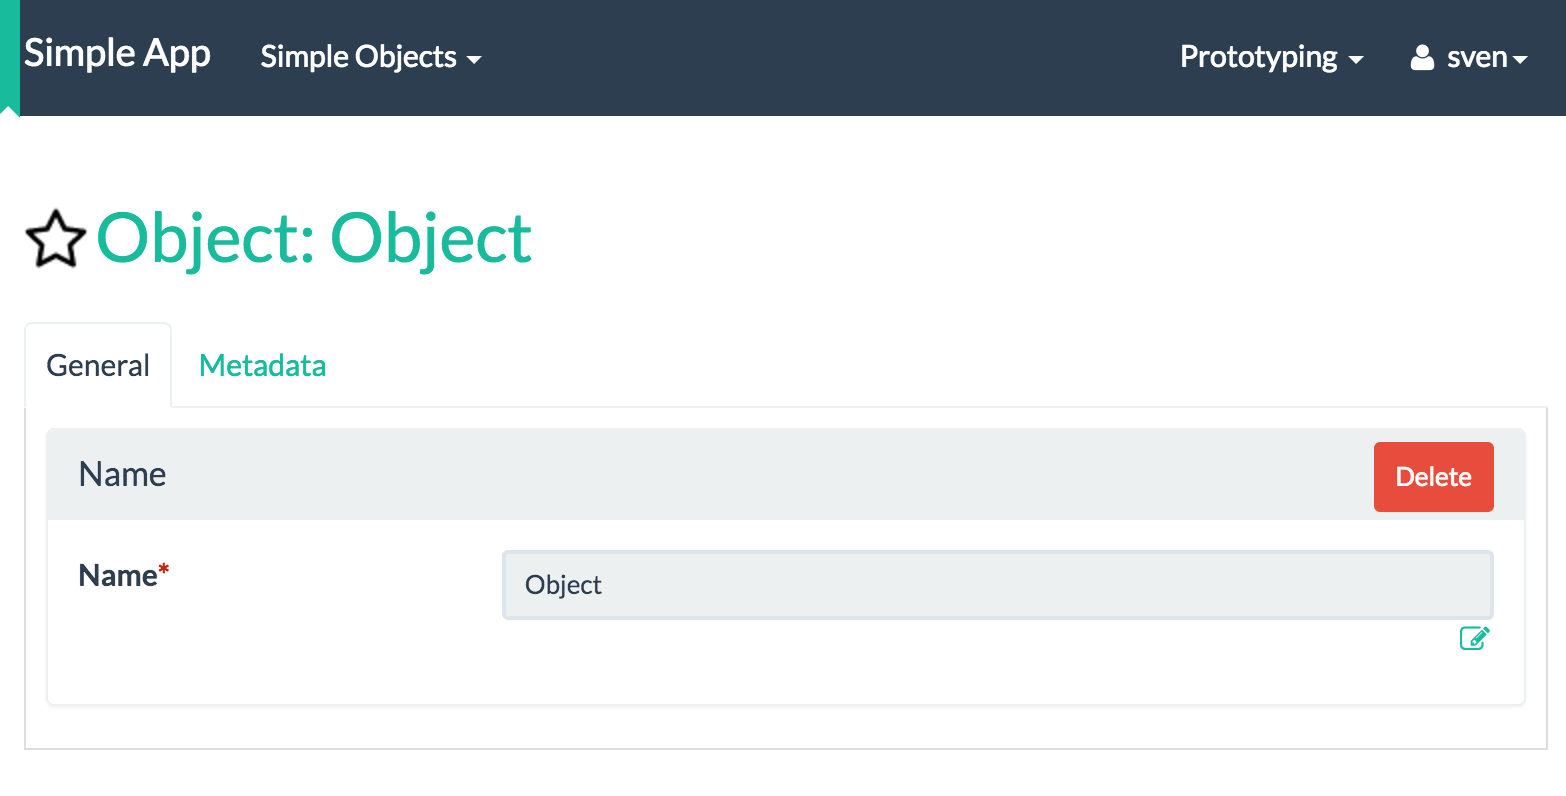
\includegraphics[width=\textwidth]{figures/simpleobjectui}
\end{minipage}
\caption{A very simple example of how the user interface is derived from code}
\end{figure}

\subsection{Domain-Driven Design}
\label{subsection:domaindrivendesign}
Software projects have been riddled by failure for as long as they have been around. A 1999 survey by Linberg found that 20\% of software projects failed and another 46\% suffered from severe delays, exceeding budgets or missing functionality or a combination of the three\cite{linberg1999software}. In 2007, the Standish Group concluded that 35\% of software projects could be classified as successful, with 46\% suffering from the aforementioned problems and 19\% completely failing\cite{rubinstein2007standish}. Keil et al. concluded that a key factors in the failure of software projects are information asymmetry and goal incongruence\cite{keil2000software}.

Those exact issues are at the core of what \textit{\acrlong{ddd}} (\acrshort{ddd}), conceived by Eric Evans in 2004, encapsulates. In a business software project, there are two main parties involved: the domain experts (the business experts) and the technical experts (the developers). These parties will have to work together in order to specify the functionality of the software. Business language, however, is very different from technical language, and thus some method of translation is needed. A business analyst could provide this translation, but this only adds another layer of potential misunderstanding, ultimately culminating in faulty behaviour being implemented.

\subsubsection{Ubiquitous language}
\label{subsubsection:ubiquitouslanguage}
The first central concept in \acrshort{ddd} is to create an \textit{ubiquitous language} between the domain experts and technical experts. By clearly defining what terms to use for what concepts and ensuring that both parties understand what they mean, information asymmetry can be avoided\cite{evans2004domain}. These defined terms together form the domain model which is used to describe and specify the software. Undoubtedly, at some stage in the process the ubiquitous language will prove itself insufficient to accurately describe new functionality, which implies that the model should be expanded. This creates an iterative development process where both parties have to put in effort to be as concise as possible. It also prevents the domain model from growing too complex: if the parties fail to define a certain aspect of the model, it is highly unlikely that it will be successfully implemented in the software and it is better to leave it out.

\subsubsection{Model-driven design}
\label{subsubsection:modeldrivendesign}
Once the domain model has been specified to a sufficient extent to initiate the development process, the second central concept in \acrshort{ddd} comes to light: \textit{model-driven design}. As the name suggests, this means writing your software driven by the domain model. The domain model will function as the translation layer between the domain experts and the technical experts, as the software becomes more comprehensible for the domain experts if the software uses the same ubiquitous language. The code and domain model share a bidirectional relationship: if the domain model is extended, the code must be changed, and if the code is changed, the domain model must be adapted\cite{evans2004domain}. This prevents the issue of goal incongruence, as the domain experts and technical experts are aligned in terms of what has to be implemented. After all, the domain model is binding and defined in a collaborative effort.

\subsection{Naked Objects pattern}
\label{subsection:nakedobjectspattern}
One of the frustrations often expressed regarding \acrshort{ddd} is that while the ubiquitous language combined with the derived domain model may very well tackle the problem of goal diversion, it also increases overhead greatly. Consider figure~\ref{figure:applicationlayers}: the domain model is represented in the business logic layer. Recall that we've stated that the domain model will be refined over the course of time, and that any changes to the domain model must be reflected in the code. This means that any modifications to the domain model will have to be applied to the other layers, too.

\begin{figure}[h]
	\center
	\include*{figures/applicationlayers}
	\caption{The main application layers in \acrshort{ddd}}
	\label{figure:applicationlayers}
\end{figure}

To address this issue, Richard Pawson designed the Naked Objects pattern, based on three core concepts\cite{pawson2002naked}:
\begin{enumerate}
	\item Business logic should only reside in domain objects\footnote{A domain object is an entity that holds relevant data, in order to transfer the data between the application layers.}
	
	\item The user interface is an exact representation of the domain objects, and thus is an object-oriented user interface
	
	\item The user interface is derived completely and fully automatically from the domain objects through reflection
\end{enumerate}

These three concepts combined provide a means of developing software that robustly follows the philosophy of \acrshort{ddd}. The first two concepts ensure that the software implements the domain model and prevents the use of technical language. The application, whether prototypal or deployed, will feel familiar to the stakeholders and developers alike. The third concept is not necessarily related to \acrshort{ddd}, but does take away the burden of developing the presentation layer and thus places the focus on the business logic: i.e., the domain model.

\section{User interface migration in history}
\label{section:userinterfacemigrationinhistory}
In the history of user interfaces, two events stand out: the migration from character-based interfaces to graphical interfaces, and implementing a web-based interface for a native application.

As the use of \acrshortpl{gui} became widespread, a lot of older software still made use of legacy user interfaces. These interfaces were usually character-based interfaces, developed for hardware that did not offer the capabilities to use a \acrshort{gui}\cite{merlo1995reengineering}. Developers quickly came to notice that the migration of one user interface to the other was not easily accomplished, as end users wanted novel user interfaces to have identical functionality as the legacy counterpart, and a lack of homogenisation in hardware support resulted in a vast amount of code refactoring to achieve the desired result\cite{moore1994knowledge}. On top of that, simply redesigning the software from scratch would be an effort too costly in terms of resources and investments. As a result, the developers often reverse engineered the system, creating an object-oriented model and then wrapping the legacy objects so that the new system could use these entities\cite{de1997migrating}. This method allowed developers to incrementally phase out parts of the software until all legacy objects were removed.

Another major shift in user interface design came to the forefront when the internet was adopted in offices and homes alike and applications started to become available in the web browser rather than a native application for independent operating systems. This migration is still taking place to this day; an example is Skype, of which Microsoft introduced a preview version of its web based version as late 2013\cite{TypeL20:online}. Developers now had to deal with writing the presentation layer in all-new web technologies which run client side, while respecting the many constraints dictated by the software. When the underlying logic is not too complex, developers usually opted for "grafting" the web interface on top of the application, designing most of the mutually indepent functionalities from scratch and applying reverse engineering where necessary. For more complex applications, however, a comparable wrapping method as mentioned before could also be employed\cite{aversano2001migrating}.

Developers often also face the common issue of "dead" or "glue" code when migrating legacy systems to a web version, requiring the developers to thoroughly analyse code to prevent obsolete functionality from being implemented in the new user interface. Moreover, partially reusing code modules may also violate application logic\cite{stroulia2003user}. Finally, the great advantage of web availability of software is that it becomes accessible to a vast group of users: e.g. a bank offering web-based banking to its customers, removing the need of trained bank clerks. This does, however, introduce another layer of complexity, as the various groups of users should interact with the user interfaces designed for them - corporate clients require more functionality than a personal customer, but they both speak to the same back end\cite{aversano2001migrating}.